\documentclass[12pt]{article}
\usepackage{amsmath, amssymb}
\usepackage{geometry}
\geometry{margin=1in}
\usepackage{xcolor}
\usepackage{tikz}
\usetikzlibrary{arrows.meta, positioning, calc, decorations.markings}

\definecolor{cold}{RGB}{60,100,180}
\definecolor{warm}{RGB}{200,80,40}
\definecolor{mid}{RGB}{80,150,120}
\definecolor{dim}{RGB}{160,160,160}
\definecolor{gnd}{RGB}{230,220,200}

\title{Brain}
\author{Diego Rincón}
\date{}

\begin{document}
\maketitle

\section*{State}

A brain is a weighted directed graph $G = (V, E, w)$ where each node
$v \in V$ carries a state $x_v \in \mathbb{R}$ and each edge
$(u,v) \in E$ carries a weight $w_{uv} \in \mathbb{R}$.

Update rule (discrete time):
\[
x_v(t+1) = \sigma\!\left(\sum_{u \to v} w_{uv}\, x_u(t) + b_v\right)
\]
where $\sigma$ is a nonlinearity and $b_v$ is a bias.

Ground state: $x^* = \sigma(Wx^* + b)$, a fixed point.

\bigskip

\begin{center}
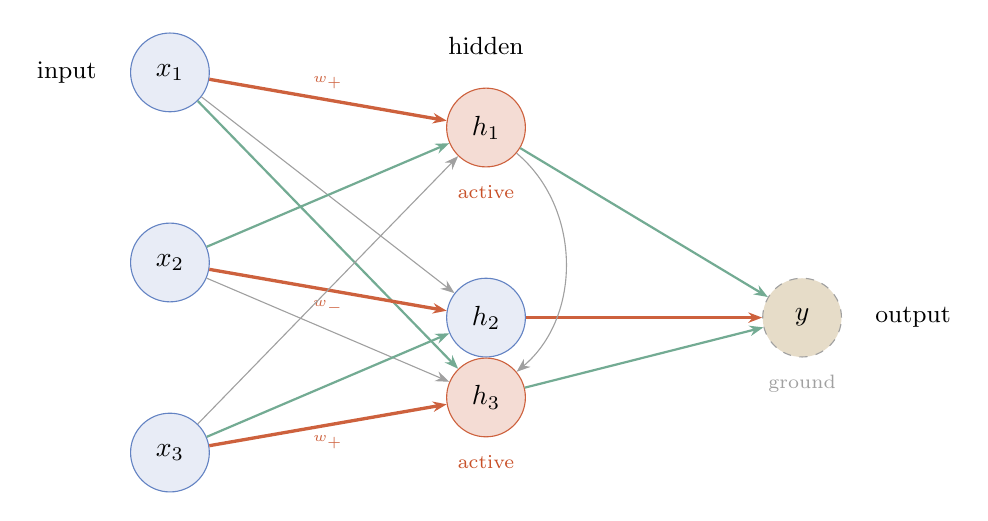
\begin{tikzpicture}[
  node distance=2.2cm,
  neuron/.style={circle, draw=cold!80, fill=cold!12, minimum size=1cm, inner sep=0},
  active/.style={circle, draw=warm!90, fill=warm!20, minimum size=1cm, inner sep=0},
  ground/.style={circle, draw=dim, fill=gnd, minimum size=1cm, inner sep=0, dashed},
  arr/.style={-{Stealth[length=5pt]}, thick, mid!80},
  strong/.style={-{Stealth[length=5pt]}, very thick, warm!90},
  weak/.style={-{Stealth[length=5pt]}, thin, dim},
]

% Input layer
\node[neuron] (i1) {$x_1$};
\node[neuron, below=1.4cm of i1] (i2) {$x_2$};
\node[neuron, below=1.4cm of i2] (i3) {$x_3$};

% Hidden layer
\node[active, right=3cm of i1, yshift=-0.7cm] (h1) {$h_1$};
\node[neuron, right=3cm of i2, yshift=-0.7cm] (h2) {$h_2$};
\node[active, right=3cm of i3, yshift=0.7cm] (h3) {$h_3$};

% Output
\node[ground, right=3cm of h2] (o1) {$y$};

% Input -> Hidden
\draw[strong] (i1) -- (h1) node[midway, above, font=\tiny] {$w_{+}$};
\draw[weak]   (i1) -- (h2);
\draw[arr]    (i1) -- (h3);

\draw[arr]    (i2) -- (h1);
\draw[strong] (i2) -- (h2) node[midway, below, font=\tiny] {$w_{-}$};
\draw[weak]   (i2) -- (h3);

\draw[weak]   (i3) -- (h1);
\draw[arr]    (i3) -- (h2);
\draw[strong] (i3) -- (h3) node[midway, below, font=\tiny] {$w_{+}$};

% Hidden -> Output
\draw[arr]    (h1) -- (o1);
\draw[strong] (h2) -- (o1);
\draw[arr]    (h3) -- (o1);

% Recurrent connection on h1
\draw[weak, bend left=50] (h1) to (h3);

% Labels
\node[left=0.3cm of i1, font=\small] {input};
\node[above=0.3cm of h1, font=\small] {hidden};
\node[right=0.3cm of o1, font=\small] {output};

% State annotations
\node[below=0.1cm of h1, font=\scriptsize, text=warm] {active};
\node[below=0.1cm of h3, font=\scriptsize, text=warm] {active};
\node[below=0.1cm of o1, font=\scriptsize, text=dim] {ground};

\end{tikzpicture}
\end{center}

\bigskip

\section*{Ground}

The network reaches ground when $\|x(t+1) - x(t)\| < \varepsilon$.
Silence is the attractor. Activation is displacement from it.

Energy:
\[
E(x) = -\frac{1}{2} x^\top W x - b^\top x
\]
Hopfield form. Decreases monotonically under asynchronous update
when $W = W^\top$.

\section*{The Adaptive Connection}

Each weight $w_{uv}$ is adaptive:
\[
w_{uv}(t+1) = w_{uv}(t) - \alpha \frac{\partial E}{\partial w_{uv}}
\]
Large $\alpha$: fast forgetting, near ground. Small $\alpha$: memory persists.
At $\alpha = 0$: frozen weights, fixed character.

\end{document}
